%% LaTeX2e class for student theses
%% sections/content.tex
%% 
%% Karlsruhe Institute of Technology
%% Institute of Information Security and Dependability
%% Software Design and Quality (SDQ)
%%
%% Dr.-Ing. Erik Burger
%% burger@kit.edu
%%
%% Version 1.6, 2024-06-07

\chapter{Concept}
\label{ch:Concept}
%/ Using TGGs to define Consistency Preservation Rules
To be able to utilize TGGs for defining consistency preservation rules in \textsc{Vitruvius}, a transformation process from sequences of atomic changes from the \textsc{Vitruvius} change metamodel (see \autoref{sec:Foundations:Vitruvius}) to applications of TGG rules has been developed, and a prototype has been implemented.

In \textsc{Vitruvius}, all changes are atomic or composite, with composite changes being a sequence of atomic changes. \enquote{atomic} is defined by Klare et al. \cite{VitruviusKlare2021} as affecting \enquote{only one element value}. 
TGG rule applications differ from \textsc{Vitruvius} changes insofar as pattern applications can affect more than one model element and are intended to be able to express complex relationships in consistency definitions in the change model.

In the context of using that ability of TGGs for \textsc{Vitruvius}, this gives rise to the question of how those atomic \textsc{Vitruvius} changes can be accurately mapped to complex TGG rule applications and the question of how TGG rules can be represented to enable this mapping.
In this thesis, these questions were investigated by developing and researching existing strategies for correctly detecting complex patterns in atomic change sequences and applying them to the given use case and/or developing new strategies.

\begin{figure}
\centering
\includegraphics[width=15cm]{figures/concept-overview.pdf}
\caption{An Overview of the transformation process concept.}
\label{fig:ConceptOverview}
\end{figure}

\autoref{fig:ConceptOverview} gives an overview of the transformation process concept. A sequence of atomic \textsc{Vitruvius} changes to a source model, recorded by a change monitor or derived from state differences (both being existing \textsc{Vitruvius} functionality) is given, as well as a source and a target model. The process transforms the given sequence to a sequence of TGG source rule applications. The source rule definitions are derived from TGG rule definitions. The source rule application sequence is used to synchronize the target model. Since TGG source rules map to target rules because both are derived from a single TGG rule, the source rule application sequence can be mapped to a target rule application sequence, which is then used by the TGG engine to synchronize the target model.
For full \textsc{Vitruvius} integration, the target rule application sequence can be transformed to a sequence of atomic \textsc{Vitruvius} changes to the target model, which is not done by the TGG engine but by the conversion process. However, that step is not covered by the implemented prototype.


% A strategy for converting atomic change sequences to TGG rule application sequences has to group changes together, so that a pattern may be applicable to the resulting composite change.
% Especially picking changes out-of-order is necessary to identify patterns. 

In the remainder of this chapter, the developed concepts and algorithms to realize the process of converting \textsc{Vitruvius} change sequences to TGG rule applications are described.

The foundational concept is called \emph{Backward-Conversion Pattern Matching}.
The first section (\autoref{sec:Concept:BackwardConversionPM}) describes the core of this concept, and the sections \autoref{sec:Concept:BackwardConversionPM:GreenMatching} and \autoref{sec:Concept:BackwardConversionPM:BlackMatching} its realization in detail.
Further sections consider concepts and algorithms that solve necessities that Backward-Conversion Pattern Matching introduces if one does not want to fall back to using a solely graph-based pattern matcher.

% ---------------------------------------------------------------------------------------------------------------------------
% ---------------------------                Backward Conversion Pattern Matching                 ---------------------------
% ---------------------------------------------------------------------------------------------------------------------------
\section{Backward-Conversion Pattern Matching: Overview}
\label{sec:Concept:BackwardConversionPM}
In this thesis, the foundational concept for solving the problem of generating TGG rule application sequences out of \textsc{Vitruvius} change sequences is to transform the problem to the Vitruvius change space and solve it there. 
It involves converting TGG patterns to template sequences of atomic \textsc{Vitruvius} changes and matching those template sequences in a change sequence given by \textsc{Vitruvius}. 
In the following, this concept is briefly outlined.

\begin{figure}
\centering
\includegraphics[width=15cm]{figures/tggRule_methodClassParamTypeToParamType.pdf}
\caption[Running Example \emph{MethodClassParamTypeToParamType}]{Running Example \emph{MethodClassParamTypeToParamType}: A triple graph grammar rule describing a consistency relationship between typing of method parameters in Java and UML. Green nodes and edges indicate the right-hand side of the rule, i.e. what is added to both models.}
\label{fig:tggRule_methodClassParamTypeToParamType}
\end{figure}


\begin{figure}
\centering
\includegraphics[width=15cm]{figures/Backward-Conversion-Pattern-Matching.pdf}
\caption[Data flow in the Backward Conversion Pattern Matching concept]{Activity Diagram, giving an Overview of data flow in the Backward Conversion Pattern Matching concept, from change sequence retrieval to applying TGG rules in the target model. The orange nodes mark the process steps of the concept. Arrow labels in \texttt{[brackets]} indicate control flow, other labels indicate data flow.}
\label{fig:BackwardConversionPatternMatching}
\end{figure}

Imagining the whole process as a pipeline, depicted in \autoref{fig:BackwardConversionPatternMatching}, the conversion of TGG rules to templates that are mappable to change sequences, this step can be seen as a step backwards, thus it is called \emph{backward conversion}.
Backward conversion identifies the \emph{green} nodes and edges (see \autoref{fig:tggRule_methodClassParamTypeToParamType}) of the source or the target side of a TGG rule, maps them to \textsc{Vitruvius} \emph{EChange} classes, and builds a data structure that preserves the graph structure implicitly and is mappable to changes from a change sequence.
Section \ref{sec:Concept:BackwardConversionPM:BackwardConversion} describes the algorithm and the data structure in more detail.

Upon having converted TGG rules to change sequence templates, \emph{green matching} can be performed. This is called green matching because only the \emph{create} nodes and edges, also called green nodes and edges, that a TGG rule contains are considered here.
The reason for not also considering the (black) context nodes at this point is that context is partly existing prior to the pattern matching process, but also partly arising in the process. So, matching context prematurely would prevent finding matches whose context is created at the time of pattern matching.
In \autoref{sec:Concept:BackwardConversionPM:GreenMatching}, the process of invoking change sequence templates upon change sequences and covering the sequences with such invocations is described.

After receiving change sequence template applications from green pattern matching, each of these is tried to be matched fully, meaning that, in addition to the green nodes already matched, black nodes are matched against model elements, too.
Because applying a black-matched TGG rule application to the target model can enable other change sequence template applications to be matchable, this process is done repeatedly until there are no more new TGG rule applications.
Section \ref{sec:Concept:BackwardConversionPM:BlackMatching} describes the algorithm of completing a green match by trying to map the context nodes that remain unmatched after green matching.
This requires a graph-based approach that traverses both source model and TGG rule alongside, recursively extending the mapping of TGG rule node to source model node that was created by green matching.

Between black pattern matching and applying the fully matched TGG rule application to the target model, pattern selection is performed, which is described in \ref{sec:Concept:PatternSelection}. This is necessary because there might be multiple rule applications covering one or more EChanges, and only one of those can be applied. This choice has to be made after black pattern matching, and thus, possibly multiple times, to maximize coverage and not select-out pattern applications that fail black pattern matching.

To deal with subtractive changes, red pattern matching, described in \autoref{sec:Concept:RedMatching}, is performed.
Subtractive changes invalidate previously applied TGG rule applications, but this might also result in other EChanges being covered by a rule application no more. Thus, first detecting which TGG rule applications are now invalid, these \enquote{freed} EChanges are detected, re-created, and added to the other additive changes given by the currently recorded changes to the source model.

\section{Backward Conversion: Making TGG patterns matchable to change sequences}
\label{sec:Concept:BackwardConversionPM:BackwardConversion}
To be able to base the pattern matching of TGG rules to model changes on \textsc{Vitruvius} change sequences, in this section, the idea and conceptual realization of \emph{backward conversion} of TGG rules is presented. The key idea is to represent the structure of a TGG rule in the form of a template that is more easily matchable to a sequence of atomic changes than trying the same with a graphically represented TGG rule would be. To that end, the idea of extracting the change information of green nodes and edges and building a data structure that represents these changes and their interrelation in a form that resembles a collection of \textsc{Vitruvius} \emph{EChanges}, that are not initialized with actual elements but with placeholders that bind these changes together was created and is elaborated in the following.

For matching TGG rules to sequences of changes that have occurred in a model, only that side of the TGG rules that has the same metamodel as the model in which the changes have taken place is needed for backward conversion and green matching.
To be able to match TGG rules to sequences of changes of the \textsc{Vitruvius} change metamodel(\emph{EChanges}), a custom data structure is defined that serves as the output of the \emph{Backward Conversion} process.
In the following, this data structure is described. After that, the algorithm that parses a TGG rule into this data structure is presented.
\autoref{fig:ChangeSeqTemplateWrappersPlaceholder} shows how the \emph{Change Sequence Template} data structure is constructed, and in \autoref{fig:tggRule_methodClassParamType_Templated}, an instance example can be seen.

\begin{figure}
\centering
\includegraphics[width=15cm]{figures/ChangeSeqTemplateWrappersPlaceholder.pdf}
\caption[Change Sequence Templates, EChangeWrappers and EObjectPlaceholders]{Change Sequence Templates, EChangeWrappers and EObjectPlaceholders are used to represent a TGG rule in a way that makes it more conveniently matchable to a sequence of atomic \textsc{Vitruvius} changes. EObjectPlaceholders are contained in possibly more than one EChangeWrapper, sometimes as \emph{affectedElement}, sometimes as \emph{value}.
To be able to apply Change Sequence Templates more than once, they are copyable.}
\label{fig:ChangeSeqTemplateWrappersPlaceholder}
\end{figure}

\begin{figure}
\centering
\includegraphics[width=15.5cm]{figures/tggRule_methodClassParamType_Templated.pdf}
\caption[Running Example \emph{MethodClassParamTypeToParamType} with template representation]{Running Example \emph{MethodClassParamTypeToParamType}. The colored graph at the top shows the source graph of a triple graph grammar rule. Bottom graph: Instance diagram of the converted source graph in the Change Sequence Template data structure.}
\label{fig:tggRule_methodClassParamType_Templated}
\end{figure}

\paragraph{Change Sequence Templates} \emph{Change Sequence Templates} represent one converted rule. They consist of EChange wrappers, that hold the type of EChange they represent plus one or multiple placeholders for actual EChanges.
\emph{EChange Wrappers} each represent one atomic EChange class of the \textsc{Vitruvius} change metamodel that might occur in a change sequence. They also represent one green node or edge in the rule pattern of the change sequence template they belong to.
Depending on the type of EChange that is represented, an EChange wrapper holds different numbers of \emph{Placeholders}. This is exemplarily shown in \autoref{fig:tggRule_methodClassParamType_Templated}.
Each placeholder stands for an actual object that is concerned by possibly more than one EChange.
If more than one EChange concerns the same EObject, that EObject will still only be represented by one placeholder, which then occurs in multiple EChange wrappers.
In that way, placeholders ensure that the graph structure of the TGG rule is retained throughout the conversion process.

The process of converting a TGG rule to generate a change sequence template is realized via a depth-first search through the TGG rule graph.

% \begin{algorithm}
%     \caption{Backward Conversion: Depth-first search}
%     \label{alg:backwardConversion:DFS}
%     \begin{algorithmic}
%     % \Require{Write here the required data}
%     % \Ensure{Write here the expected result}
%         \State $eChangeWrappers \gets \Call{HashSet}{}$
%         \State $graphElementsVisited \gets \Call{HashSet}{}$
%         \newline
%         \Function{convertRule}{$rule: TGGRule$}
%             \State $eChangeWrappers \gets \Call{HashSet}{}$
%             \State $graphElementsVisited \gets \Call{HashSet}{}$
%             \ForAll{$ruleNode : rule.contextNodes$}
%                 \State $\Call{parseContextNode}{ruleNode}$
%                 \Comment{Recurse, skipping context nodes and}
%                 \State 
%                 \Comment{edges until a create node or edge}
%             \EndFor
%             \ForAll{$ruleNode : rule.createNodes$}
%                 \State $\Call{parseCreateNode}{ruleNode}$
%             \EndFor
%             \State \Return{$\Call{ChangeSequenceTemplate}{eChangeWrappers}$}
%         \EndFunction
%         \newline
%     \end{algorithmic}
% \end{algorithm}

% \begin{algorithm}
%     \caption{Backward Conversion: Placeholder and EChange Wrapper Creation}
%     \label{alg:backwardConversion:PlaceholdersAndEChangeWrappers}
%     \begin{algorithmic}
%         \Function{parseCreateNode}{$ruleNode: TGGRuleNode$}
%             \If{\Call{visited}{$ruleNode$}}
%                 \State \Return{}
%             \EndIf
%             \State $newEChangeWrapper \gets \Call{PlainEChangeWrapper}{}($
%             \State \hspace{5.2cm} $CreateEObject.EClass,$
%             \State \hspace{5.2cm} $ruleNode.representingEClass,$
%             \State \hspace{5.2cm} $\Call{getOrCreatePlaceholder}{ruleNode}$
%             \State \hspace{4.5cm} $)$
%             \State $eChangeWrappers \gets eChangeWrappers \cup newEChangeWrapper $
%             \If{\Call{hasNoIncomingContextOrCreateEdgesFromSameDomain}{$ruleNode$}}
%                 \State $newEChangeWrapper \gets \Call{PlainEChangeWrapper}{}($
%                 \State \hspace{5.2cm} $InsertRootEObject.EClass,$
%                 \State \hspace{5.2cm} $ruleNode.representingEClass,$
%                 \State \hspace{5.2cm} $\Call{getOrCreatePlaceholder}{ruleNode}$
%                 \State \hspace{4.5cm} $)$
%                 \State $eChangeWrappers \gets eChangeWrappers \cup newEChangeWrapper $
%             \EndIf
%         \EndFunction
%         \newline        
        
%         \Function{parseCreateEdge}{$ruleEdge: TGGRuleEdge$}
%             \State $referenceType \gets ruleEdge.EReference$
%             \State $affectedElementType \gets ruleEdge.sourceNode.representingEClass$
%             \State $affectedElementPlaceholder \gets \Call{getOrCreatePlaceholder}{ruleEdge.sourceNode}$
%             \State $valuePlaceholder \gets \Call{getOrCreatePlaceholder}{ruleEdge.targetNode}$
%             \State $newEChangeWrapper \gets \Call{EReferenceValueIndexEChangeWrapper}{}($
%             \State \hspace{5.2cm} $InsertEReference.EClass,$
%             \State \hspace{5.2cm} $affectedElementType,$
%             \State \hspace{5.2cm} $affectedElementPlaceholder,$
%             \State \hspace{5.2cm} $referenceType,$
%             \State \hspace{5.2cm} $valuePlaceholder$
%             \State \hspace{4.5cm} $)$
%             \State $eChangeWrappers \gets eChangeWrappers \cup newEChangeWrapper $
%             \State $\dots$
%             \Comment{Continue DFS \dots}
%         \EndFunction
%         \newline
        
%         \Function{getOrCreatePlaceHolder}{$ruleNode: TGGRuleNode$}
%             \If{\Call{alreadyHasPlaceholder}{$ruleNode$}}
%                 \State \Return{\Call{getPlaceholder}{$ruleNode$}}
%             \Else
%                 \State \Return{\Call{createAndMapToPlaceholder}{$ruleNode$}}
%             \EndIf
%         \EndFunction
%     \end{algorithmic}    
% \end{algorithm}

% Noteworthy parts of the algorithm are shown in \autoref{alg:backwardConversion:DFS} and \autoref{alg:backwardConversion:PlaceholdersAndEChangeWrappers}.
The algorithm visits the green nodes and edges of the rule, and parts of its direct neighborhood consisting of context nodes that are connected to green nodes via green edges. In that case, the context node is modified, so it must be taken into consideration.

For green nodes, one $PlainEChangeWrapper$ is created based on the $EClass$ that the green node represents and typed as a $CreateEObject$.
Further, the wrapper is given a placeholder, that is created if there is none already existing for the node.
If a green node does not have any incoming context or create edges in the same domain (source or target, depending on which is currently looked upon), that is interpreted as the creation of a root node in the model, so a second $PlainEChangeWrapper$ is created and typed as an $InsertRootEObject$. Placeholder and $EClass$ of the affected EObject stay the same as with the other wrapper.

In the case of a green edge, an $EReferenceValueIndexEChangeWrapper$ is created, typed with $InsertEReference$. It is given the EClass that the source node of the edge represents, the placeholder of the source node, the EReference that the edge represents, and a placeholder for the value that is inserted into the reference.

\section{Green Pattern Matching: Additive Changes}
\label{sec:Concept:BackwardConversionPM:GreenMatching}
After Change Sequence Templates are created, a change sequence can be matched against those templates to detect the complex patterns that form the precondition for applying the TGG rule, i.e. consistency preservation rule.
In this section, the algorithm to partly and fully invoke Change Sequence Templates by traversing the change sequence is given and described.
A match found by this algorithm does not automatically mean that it is really applied, since context matching (see \autoref{sec:Concept:BackwardConversionPM:BlackMatching}) and pattern selection (see \autoref{sec:Concept:PatternSelection}) sort out matches.

The algorithm can be seen in \autoref{alg:BackwardConversionPM:GreenPatternMatchingMain} and works in the following way:
For each change of the given change sequence, it generates all possible partly initialized invocations of change sequence templates for that EChange. If some are duplicates of template invocations generated in previous loop iterations, these are discarded. The remaining invocations are globally stored to keep the result and for duplicate detection.
Then, each of these  template invocations is tried to be fully matched against the other EChanges of the change sequence.
To that end, each EChangeWrapper contained in the currently treated template invocation
is tried to be matched with each EChange that comes into question until a match is found.
These EChange candidates are determined by whether their EChange type matches the EChangeWrapper's type.
Matching is performed by checking whether the types of the EObjects and, e.g., the EReference contained in the EChange match the types expected in the EChangeWrappers. 

In the following, helper functions that are not written in pseudocode are described:

\textsc{rememberWrappersInvokedWithEChange} takes an EChange and a set of templates partly initialized with the given EChange.
For each partly initialized template invocation, the function finds the EChangeWrapper that has been initialized with the given EChange and remembers, globally, that the original (see \autoref{fig:ChangeSeqTemplateWrappersPlaceholder}) of that EChangeWrapper has been invoked with the given EChange. This allows for removing duplicates with \textsc{removeDuplicateTemplateInvocations}.

\textsc{rememberWrapperInvokedWithEChange} takes an EChange and an EChangeWrapper that has been initialized with the given EChange.
It remembers, globally, that the original (see \autoref{fig:ChangeSeqTemplateWrappersPlaceholder}) of the given EChangeWrapper has been invoked with the given EChange. This allows for removing duplicates with \textsc{removeDuplicateTemplateInvocations}.

\textsc{removeDuplicateTemplateInvocations} takes an EChange and a set of templates partly initialized with the given EChange.
For each partly initialized template, the function checks whether the \emph{original} (see \autoref{fig:ChangeSeqTemplateWrappersPlaceholder})  of the EChangeWrapper in the template that contains the given EChange has already been invoked with the given EChange and removes the thus detected duplicates from the set.

$ChangeSequenceTemplateSet$::\textsc{invokeTemplatesByEChange} takes an eChange and returns all possible invocations of change sequence templates contained in that set.
This means each template that contains one or more EChangeWrappers that match the eChange is invoked. 
Invoked means, the template is \emph{deep copied}, which means that all EChangeWrappers and placeholders are copied, too. In the EChangeWrappers' case, the \emph{original} reference is set to the original EChangeWrapper.
If a template can be invoked more than once because multiple contained EChangeWrappers match the given eChange, multiple invocations of the same pattern, but each with a different EChangeWrappers initialized, are returned.


\begin{algorithm}
    \caption{Pattern Matching with Change Sequence Templates}
    \label{alg:BackwardConversionPM:GreenPatternMatchingMain}
    \begin{algorithmic}
        \State $changeSequenceTemplateSet \gets \Call{convertTGGRules}{\dots}$
        \State $allInvokedTemplates \gets \Call{HashSet}{}$
        \Function{getGreenMatches}{$changeSequence: Sequence<EChange>$}
            \ForAll{$eChange : changeSequence$}
                \State $partlyInitializedTemplates \gets changeSequenceTemplateSet$
                \State \hspace{1.2cm} $.\Call{invokeTemplatesByEChange}{eChange}$
                % \Comment{Invoke each template, that contains an EChangeWrapper that matches the eChange, once.}
                \State $\Call{removeDuplicateTemplateInvocations}{}(eChange,$
                \State \hspace{5.2cm} $partlyInitializedTemplates)$
                \State $\Call{rememberWrappersInvokedWithEChange}{}(eChange,$
                \State \hspace{5.2cm} $partlyInitializedTemplates)$
                \State $allInvokedTemplates.addAll(partlyInitializedTemplates)$

                \ForAll{$partlyInitializedTemplate : allInvokedTemplates$}
                    \If{$\neg \Call{tryToFullyMatch}{partlyInitializedTemplate}$}
                        \State $allInvokedTemplates.remove(partlyInitializedTemplate)$
                    \EndIf
                \EndFor 
            \EndFor 
        \EndFunction
        \newline

        \Function{tryToFullyMatch}{$partlyInitializedTemplate: ChangeSequenceTemplate$}
            \State $uninitializedWrappers \gets partlyInitializedTemplate$
            \State \hspace{5.2cm} $.uninitializedEChangeWrappers$
            \ForAll{$ eChangeWrapper : uninitializedWrappers$}
                \State $wrapperIsInitialized \gets false$
                \State $eChangeCandidates \gets eChangesByEChangeType$
                \State \hspace{5.2cm} $.get(eChangeWrapper.eChangeType)$
                \ForAll{$eChangeCandidate : eChangeCandidates$}
                    \If{$eChangeWrapper.matches(eChangeCandidate)$}
                        \State $eChangeWrapper.initialize(eChangeCandidate)$
                        \State $wrapperIsInitialized \gets true$
                        \State $\Call{rememberWrapperInvokedWithEChange}{}(eChange,$
                        \State \hspace{5.2cm} $eChangeWrapper)$
                    \EndIf
                \EndFor
                \If{$\neg wrapperIsInitialized$}
                    \State \Return{false}
                \EndIf
            \EndFor
            \State \Return{true}
        \EndFunction
    \end{algorithmic}    
\end{algorithm}


\section{Black Pattern Matching: Context}
\label{sec:Concept:BackwardConversionPM:BlackMatching}
As can be seen in \autoref{fig:tggRule_methodClassParamTypeToParamType}, a TGG rule does also consist of context nodes, also called black nodes.
Since it is necessary to match one whole side of the pattern to be able to apply the green changes on the other side, the pattern-matching algorithm described in \autoref{sec:Concept:BackwardConversionPM:GreenMatching} is not sufficient.
Thus, in this section, a context-matching algorithm is described that starts from a successfully matched \emph{change sequence template}.
In particular, this means that this change sequence template provides a bijective mapping from green $TGGRuleNode$s to $EObjects$, if only that one match is looked upon.
The goal of black pattern matching is to expand this mapping so that it also contains all black context nodes.

To reduce complexity in the algorithm design, a data structure called \emph{MapStack} is defined. This data structure holds the aforementioned mapping from $TGGRuleNode$s to $EObjects$, but also provides stack functionality to enable the matching algorithm to branch and try different mappings.
If the algorithm comes to a branching situation, where multiple EObject candidates are possible, one after another is tried, and, in case of failure, the MapStack is set back to the state before the branching, so the next branch can be tried. The following methods of MapStack are of interest:

MapStack::\textsc{putPush} takes a \emph{key} and a \emph{value} and stores their mapping. It also remembers the key in its internal stack.

MapStack::\textsc{get} takes a \emph{key} and returns the \emph{value} to which the key is mapped.

MapStack::\textsc{removePopUntil} takes a \emph{key} and pops all keys until and including the given key from the stack. It removes them from the internal key-value mapping and returns all those keys.

The basic idea of the context matching algorithm is to start a depth-first search at each green node, in both incoming and outgoing directions,
and from there, move simultaneously in both the TGGRule graph and the graph given by the model.
Both are \enquote{sewn together} where the green nodes are mapped to EObjects, so that is an ideal starting point.
Talking from a TGG perspective, the algorithm does not stay in the source or target graph but behaves differently in the source and the target.
Without loss of generality, let \emph{source} be the TGG graph domain where the green pattern matching has taken place for this section.
In the target graph, the algorithm does ignore green nodes or edges, because those are precisely the ones that are to be created in the consistency-keeping process.
Nonetheless, context nodes have to be matched in the target graph.
To further reduce complexity, the algorithm never traverses green edges; it simply starts at each green node and only searches the black nodes and edges reachable from each of the green source nodes.
\textsc{visitNode} is called on each green node from the rule, which visits each incoming and outgoing edge, failing early if matching failed on one edge.


\textsc{visitOutgoingEdge} handles the target node of a rule edge and tries to match it to an EObject from the model. To that end, each EObject referenced by the EObject mapped to the source node and typed according to the EReference provided by the given \emph{outgoingEdge} is tried via \textsc{tryAllMatchingCandidatesFor} (see \autoref{alg:BackwardConversionPM:BlackMatching:MultipleCandidateHandling}).
Since outgoing edges always stay in the domain, the target rule nodes can either be context or create nodes. Create nodes are ignored, since they are handled by \textsc{contextMatches}, the starting point of the black matching algorithm.

\textsc{tryAllMatchingCandidatesFor} (see Algorithm \autoref{alg:BackwardConversionPM:BlackMatching:MultipleCandidateHandling}) takes a rule node and a set of EObject candidates that are to be tried out to be mapped to the given rule node.
The caller ensures that all EObject candidates are mappable to the rule node, so this function's only task is to try out the candidates by setting them as the rule node's mapping and recursing.
After each failed recursion, the state of the mapping and the marking of visited nodes is reset to the state before the recursion.

\textsc{visitIncomingEdge} (see Algorithm \autoref{alg:BackwardConversionPM:BlackMatching:IncomingEdges}) handles the source node of a rule edge and tries to match it to an EObject from the model. This is more complicated than visiting outgoing edges, because incoming edges can either be from the same domain or from the correspondence graph.
If the incoming edge is of the same domain as its target node, the procedure is similar to \textsc{visitOutgoingEdge}, but not quite the same.
Incoming edges in the Ecore model can either be \emph{containments} or \emph{cross-references}. Cross-references have to be found first, which is what \textsc{findAllEObjectsReferencing} does. In that case, again, there can be multiple candidates, and thus \textsc{tryAllMatchingCandidatesFor} (Algorithm \autoref{alg:BackwardConversionPM:BlackMatching:MultipleCandidateHandling}) is used to try them out.
If the incoming edge is not of the same domain as its target node, its source node must be of the TGGs correspondence graph.
In that case, the correspondence node instance is tried to be found in the TGG \emph{protocol} and mapped to the source node (correspondence node).
Also, via the correspondence node instance, the related EObject in the other domain is found and mapped to its respective rule node.
That can only be a context node, since for a correspondence node instance to exist, its source and target node instances must also exist.
From that corresponding rule node, that is from the other domain, the recursion is continued.

% \begin{algorithm}
%     \caption{Black Pattern Matching}
%     \label{alg:BackwardConversionPM:BlackMatching}
%     \begin{algorithmic}
%         \State $ruleNodeToEObjectMapStack \gets mappingsFromGreenMatching$
%         \State $tggRule$
%         \Comment{Preinitialized}
%         % \State $matchingFailed \gets false$
%         \Function{contextMatches}{}
%             \ForAll{$createNode : tggRule.createNodesInSourceDomain$}
%                 \If{$\neg \Call{visitNode}{createNode}$}
%                     % \State $matchingFailed \gets false$
%                     \State \Return{false}
%                 \EndIf
%             \EndFor
%             \State \Return{true}
%         \EndFunction
%         \newline
%         \Function{visitNode}{$ruleNode : TGGRuleNode$}
%             \If{\Call{visited}{$ruleNode$}}
%                 \State \Return{true}
%             \EndIf
%             \ForAll{$incomingEdge : ruleNode.incomingEdges$}
%                 \If{$\neg \Call{visitIncomingEdge}{incomingEdge}$}
%                     \State \Return{false}
%                 \EndIf
%             \EndFor
%             \ForAll{$outgoingEdge : ruleNode.outgoingEdges$}
%                 \If{$\neg \Call{visitOutgoingEdge}{outgoingEdge}$}
%                     \State \Return{false}
%                 \EndIf
%             \EndFor
%             \State \Return{true}
%         \EndFunction
%     \end{algorithmic}    
% \end{algorithm}

% \begin{algorithm}
%     \caption{Black Pattern Matching: outgoing edges}
%     \label{alg:BackwardConversionPM:BlackMatching:OutgoingEdges}
%     \begin{algorithmic}
%         \Function{visitOutgoingEdge}{$outgoingEdge : TGGRuleEdge$}
%             \State $srcRuleNode \gets outgoingEdge.sourceNode$
%             \State $trgRuleNode \gets outgoingEdge.targetNode$
%             \If{$\Call{visited}{trgRuleNode} \lor \Call{isCreate}{trgRuleNode}$}
%                 \State \Return{true}
%             \EndIf
%             \State $srcNodeEObject \gets ruleNodeToEObjectMapStack.get(srcRuleNode)$
%             \State $ $
%             \Comment{Outgoing always are context or create edges, so here, we stay in the domain,}
%             \State $ $
%             \Comment{looking at a context edge}

%             \State $eObjectCandidates \gets \Call{getAllMatchingReferencedEObjects}{}(srcNodeEObject,$
%             \State \hspace{5.2cm} $outgoingEdge.EReference)$
%             \State \Return{$\Call{tryAllMatchingCandidatesFor}{eObjectCandidates, trgRuleNode}$}
%         \EndFunction
%     \end{algorithmic}    
% \end{algorithm}

\begin{algorithm}
    \caption{Black Pattern Matching: incoming edges}
    \label{alg:BackwardConversionPM:BlackMatching:IncomingEdges}
    \begin{algorithmic}
        \Function{visitIncomingEdge}{$incomingEdge : TGGRuleEdge$}
            \State $srcRuleNode \gets incomingEdge.sourceNode$
            \State $trgRuleNode \gets incomingEdge.targetNode$
            \If{$\Call{visited}{srcRuleNode} \lor \Call{isCreate}{srcRuleNode}$}
                \State \Return{true}
            \EndIf
            \State $trgNodeEObject \gets ruleNodeToEObjectMapStack.get(trgRuleNode)$
            \If{$incomingEdge.domain = trgRuleNode.domain$}
                \If{$incomingEdge.EReference.isContainment$}
                    % \State $trgRuleNode.eContainer.EClass$
                    % \If{$srcRuleNode.EClass = trgRuleNode.eContainer.EClass$}
                        \State $ruleNodeToEObjectMapStack.putPush(srcRuleNode, trgRuleNode.eContainer)$
                        \State \Return{$\Call{visitNode}{srcRuleNode}$}
                    % \EndIf
                \Else                
                    \State $eObjectCandidates \gets \Call{findAllEObjectsReferencing}{}(trgNodeEObject,$
                    \State \hspace{5.2cm} $incomingEdge.EReference)$
                    \State \Return{$\Call{tryAllMatchingCandidatesFor}{eObjectCandidates, srcRuleNode}$}
                \EndIf
            \Else
                \Comment{$incomingEdge$ is a CORR edge, $srcRuleNode$ is a CORR node}
                \State $correlatedRuleNode \gets \Call{getCorrelatedNode}{trgRuleNode, srcRuleNode}$
                \If{$\Call{isContext}{correlatedRuleNode}$}
                    \State $(corrNodeInstance, correlatedEObject) \gets \Call{findCorrInstance}{}($
                    \State \hspace{5.2cm} $trgNodeEObject,$
                    \State \hspace{5.2cm} $srcRuleNode,$
                    \State \hspace{5.2cm} $correlatedRuleNode)$
                    \If{$correlatedEObject$ exists}
                        % \Comment{Remember Corr instance and correlated node instance}
                        \State $ruleNodeToEObjectMapStack.putPush(srcRuleNode, corrNodeInstance)$
                        \State $ruleNodeToEObjectMapStack.putPush(correlatedRuleNode, correlatedEObject)$
                        \State \Return{$\Call{visitNode}{correlatedRuleNode}$}
                        \Comment{Switch to other domain}
                    \EndIf
                \EndIf
                \State \Return{true} \Comment{Green node in other domain. Cannot be present.}
            \EndIf
            \State \Return{true}
        \EndFunction
    \end{algorithmic}    
\end{algorithm}


\begin{algorithm}
    \caption{Black Pattern Matching: multiple candidate handling}
    \label{alg:BackwardConversionPM:BlackMatching:MultipleCandidateHandling}
    \begin{algorithmic}
        \Function{tryAllMatchingCandidatesFor}{$eObjectCandidates : Set<EObject>, ruleNode: TGGRuleNode$}
            \If{$ruleNodeToEObjectMapStack.containsKey(ruleNode)$}
                \State \Return{$\Call{visitNode}{ruleNode}$}
            \EndIf
            
            \ForAll{$eObjectCandidate : eObjectCandidates$}
                \State $ruleNodeToEObjectMapStack.putPush(ruleNode, eObjectCandidate)$
                \If{$\Call{visitNode}{ruleNode}$}
                    % \State $matchingFailed \gets false$
                    \State \Return{true}
                \EndIf
                \State $ $
                \Comment{After each failed descend, reset visit markers and the mapping}
                \State $\Call{unmarkVisited}{ruleNodeToEObjectMapStack.removePopUntil(ruleNode)}$
            \EndFor
            \State \Return{false}
        \EndFunction
    \end{algorithmic}    
\end{algorithm}


% ---------------------------------------------------------------------------------------------------------------------------
% --------------------------------------                Match Selection                 -------------------------------------
% ---------------------------------------------------------------------------------------------------------------------------
\section{Match Selection}
\label{sec:Concept:PatternSelection}

As there might be rule matches that overlap in what they cover from the change sequence, a selection of matches becomes necessary to choose which rule match should be applied. As described in \autoref{sec:Foundations:ComplexChangeDetection}, Khelladi et al. \cite{khelladi_detecting_complex_changes_2015} introduced heuristics for that which are modified and extended in this thesis. 
The containment level heuristic is modified to be usable with a dynamic ruleset, the \emph{distance heuristic} is used as-is, and a third heuristic called \emph{max coverage} is added to account for one of this work's goals, which is preserving consistency .
The combination of these heuristics, the modification of the containment level heuristic, and the idea of the max coverage heuristic is described in the following.

\begin{figure}
\centering
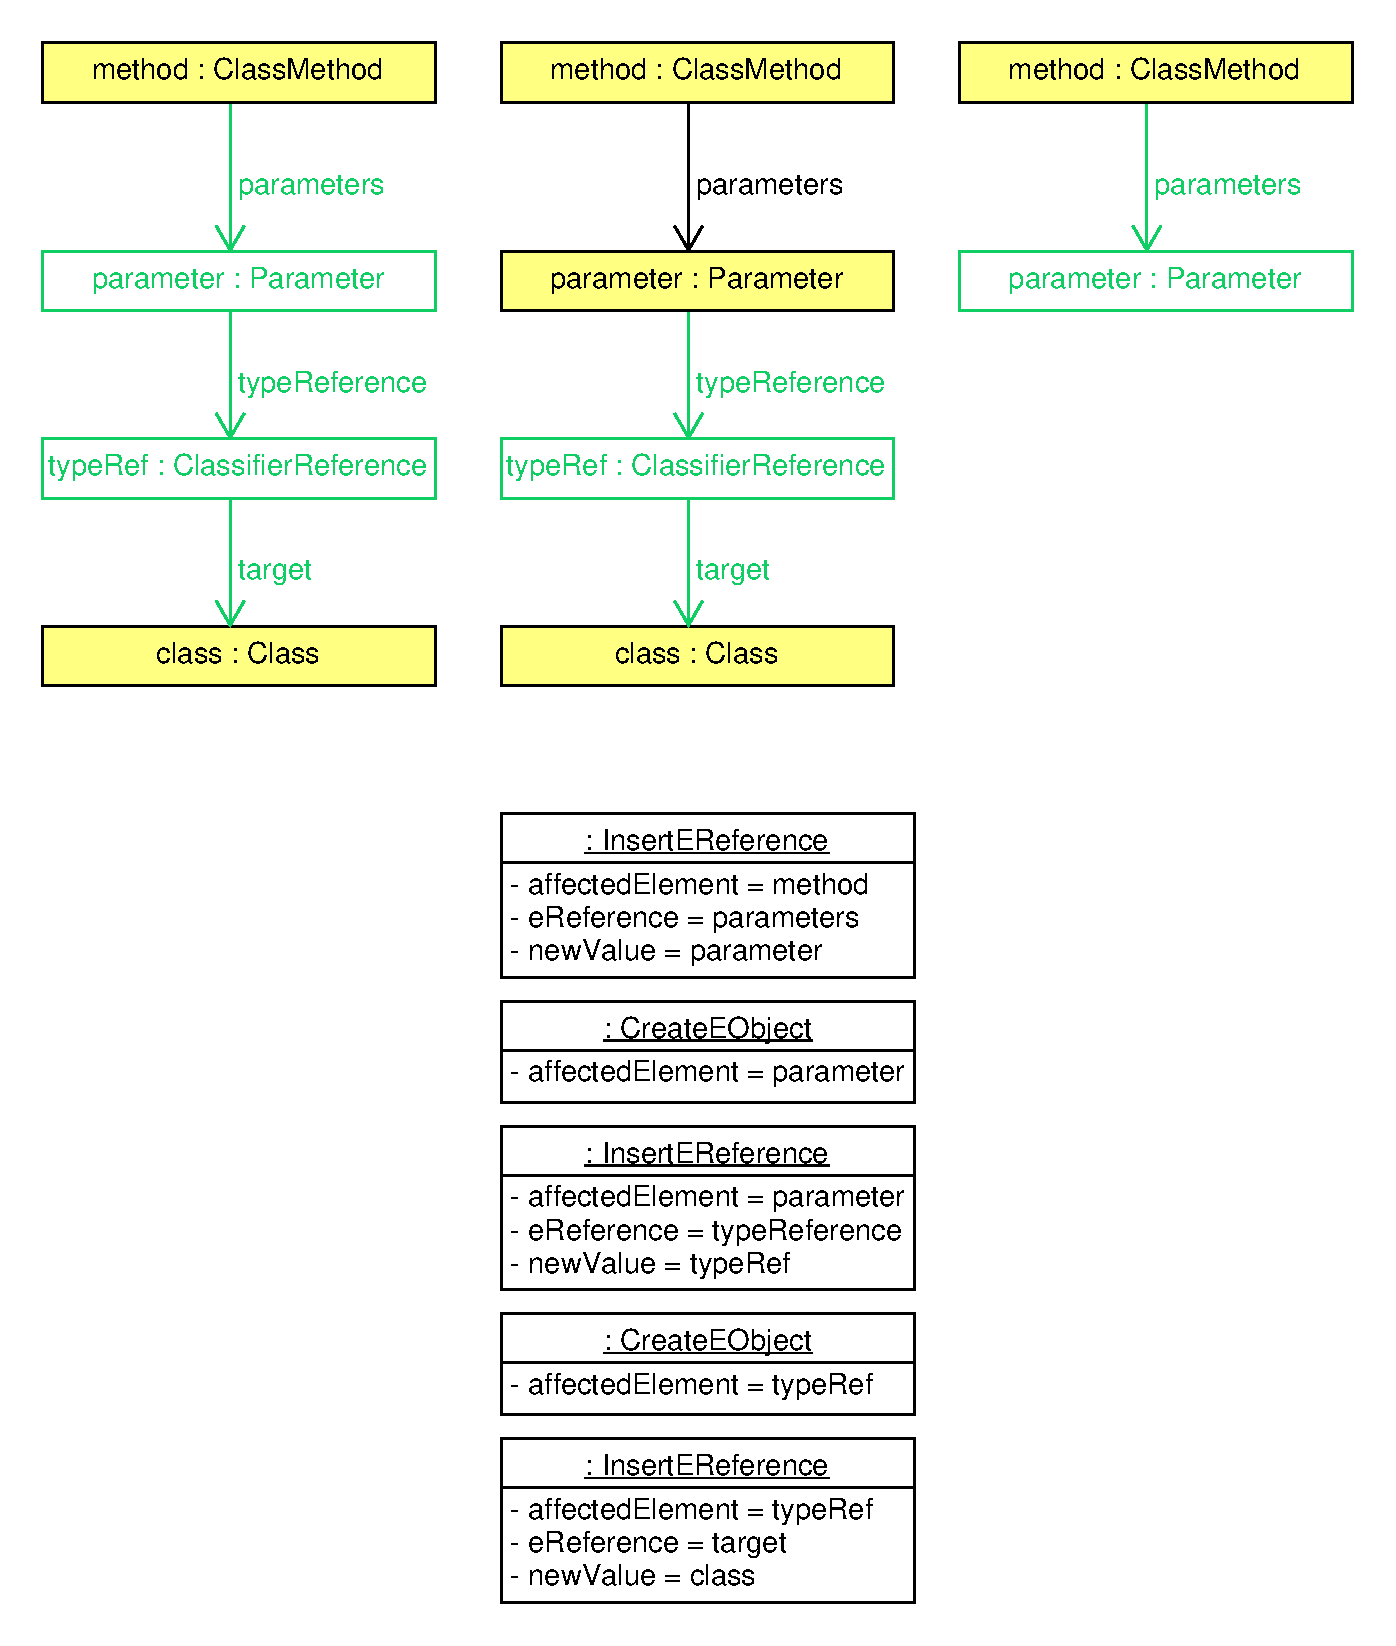
\includegraphics[width=15.8cm]{figures/tggRule_methodClassParamType_containmentExample.pdf}
\caption[Application example for the containment level heuristic]{Application example for the containment level heuristic: In the top, three source parts of TGG rules are shown. The left rule fully contains both other rules. Green matching, applied to the change sequence at the bottom of the figure, will invoke all three rules.
The dynamic containment level heuristic application algorithm will select the leftmost rule, since it contains the other two.}
\label{fig:MethodClassParamTypeContainmentExample}
\end{figure}

As envisaged by Khelladi et al. \cite{khelladi_detecting_complex_changes_2015}, this concept uses more than one heuristic at a time:
The \emph{containment level heuristic} is used first. It is modified to detect the containment level dynamically, not by pre-calculated levels, since that is not possible with a dynamic number and structure of TGG rules. In \autoref{fig:MethodClassParamTypeContainmentExample}, an application example for the containment level heuristic is shown.

Since the containment level heuristic only solves those overlap cases where one rule match completely covers another, two other heuristics are applied for the remaining conflicts. First, since it is a goal of this thesis to preserve consistency completeness, the matches with the highest coverage in the change sequence are chosen, with the intention to minimize the number of leftover EChanges that could have been matched. 
For all remaining conflicts, the \emph{distance heuristic} is used as defined by Khelladi et al. \cite{khelladi_detecting_complex_changes_2015}.

The dynamic containment level heuristic is applied as follows:
First, rule matches are sorted by the number of EChanges they cover in ascending order.
Then, for each rule match $r_i$, each rule match $r_j$ that covers more EChanges than $r_i$ is checked for containment. If $r_i$ is contained in $r_j$, $r_i$ is discarded.

% Algorithm \autoref{alg:RedMatching:DynamicContainmentLevelHeuristic} describes the application of the containment level heuristic.

% \begin{algorithm}
%     \caption{Dynamic Containment Level Heuristic}
%     \label{alg:RedMatching:DynamicContainmentLevelHeuristic}
%     \begin{algorithmic}
%         \Function{applyContainmentLevelHeuristic}{$ruleMatches$}
%             \State $sortedRuleMatches \gets \Call{sortByNumberOfEChangesAscending}{ruleMatches}$
%             \State $it \gets sortedRuleMatches.\Call{iterator}{ }$
%             \While{$it.\Call{hasNext}{ }$}
%                 \State $ruleMatch \gets it.\Call{next}{ }$
%                 \If{$it.\Call{hasNext}{ }$}
%                     % \ForAll{$containerCandidate : sortedRuleMatches.\Call{subList}{it.\Call{nextIndex}{}, n}$}
%                     \ForAll{$containerCandidate : sortedRuleMatches.\Call{subList}{it.nextIndex(), n}$}
%                         \If{$\Call{isContainedIn}{ruleMatch, containerCandidate}$}
%                             \State $ruleMatches.\Call{remove}{ruleMatch}$
%                         \EndIf
%                     \EndFor
%                 \EndIf
%             \EndWhile
%             \State \Return{$eChanges$}
%         \EndFunction
%         \newline
        
%         \Function{isContainedIn}{$potentialContainee, potentialContainer$}
%             \State $containeeEChanges \gets potentialContainee.\Call{getEChanges}{ }$
%             \State $containerEChanges \gets potentialContainer.\Call{getEChanges}{ }$
%             \State \Return{$containerEChanges.\Call{containsAll}{containeeEChanges}$}
%         \EndFunction
%     \end{algorithmic}    
% \end{algorithm}

% ---------------------------------------------------------------------------------------------------------------------------
% ---------------------------------------                RED Matching                 ---------------------------------------
% ---------------------------------------------------------------------------------------------------------------------------
\section{Red Matching: Subtractive Changes}
\label{sec:Concept:RedMatching}

In the previous sections, handling \emph{additive} EChanges that \emph{add} something to a source model and how to transport that to the target model has been covered.
However, in this concept, handling \emph{subtractive} EChanges that remove something from the model also is considered.

The \textsc{Vitruvius} change metamodel (see \autoref{sec:Foundations:Vitruvius}) also includes EChanges that are both additive and subtractive, the subclasses of \emph{ReplaceSingleValuedFeatureEChange}.
These EChanges remove the old value of an attribute or reference of an EObject and add a new value to them.
This poses a problem if one wants to map this kind of change to TGG rule applications.
In the TGG context, this change is not atomic, so this concept's approach is to split each \emph{ReplaceSingleValuedFeatureEChange} into an additive and a subtractive EChange. In the case of \emph{ReplaceSingleValuedEReference}, these are \emph{InsertEReference} and \emph{RemoveEReference}.
This split is done at the very beginning of the change propagation process, before green pattern matching.

In the following, the concept for detecting subtractive changes and repairing the TGG rule application protocol based on an atomic change sequence is described.
Without loss of generality, in this section, the assumption that the change sequence contains changes to the source model/graph is made.
Handling subtractive changes in TGGs means that we need to find out which previously applied TGG rule matches are broken because of a change to the source model.
Subsection \ref{sec:Concept:RedMatching:Implicit} and \autoref{sec:Concept:RedMatching:Explicit} describe how that detection is realizable by looking at the TGG rule application protocol and the given atomic change sequence.
Considering repair, a common strategy is to invalidate these rule applications and, cascadingly, the rule applications that have context nodes that the now-invalidated rule applications have created.
As described in \autoref{sec:Foundations:TGGs}, the concept of short-cut rules \cite{fritsche_short-cut-theoretical_2018, fritsche_short-cut-rules-repair-tgg_2021, fritsche_higher_order_short_cut_rules_2023} can be used to avoid this invalidation strategy in some cases, but not in all. Thus, the remaining cases must be dealt with.
Invalidating TGG rule applications leaves nodes and edges in the source graph uncovered by matches that potentially could be covered.
This problem is tried to be solved by re-creating EChanges from the invalidated rule applications, which is described in \autoref{sec:Concept:RedMatching:Repair}, and performing the pattern matching described in \autoref{sec:Concept:BackwardConversionPM}.

\subsection{Implicit Detection}
\label{sec:Concept:RedMatching:Implicit}
The detection of broken matches is split into implicit and explicit detection.
Implicit detection is based on the idea that each rule application recorded in the protocol that is missing a node is obviously broken.
If one assumes the change detection or recording mechanism that produces the change sequence given by \textsc{Vitruvius} is correct, this means that EChanges typed with \emph{DeleteEObject} are covered with this process.

\subsection{Explicit Detection}
\label{sec:Concept:RedMatching:Explicit}
Explicit detection means that each \emph{subtractive} EChange in the given atomic change sequence is looked upon, except \emph{DeleteEObject} and \emph{ReplaceSingleValuedFeatureEChange}. The former is covered in \autoref{sec:Concept:RedMatching:Implicit}, the latter cannot occur because, as described before, these EChanges are split up into an \emph{InsertEReference} and a \emph{RemoveEReference} EChange.

Different EChanges are handled differently; the procedure is described in the following.

\paragraph{RemoveRootEObject} This change can, but does not need to, occur together with a matching \emph{DeleteEObject} EChange, so it needs to be handled separately.
From a TGG perspective, it must have the same effects on the rule match in which the affected EObject is identified with a green node.
Thus, the rule match where the affected EObject of the RemoveRootEObject EChange occurs as bound to a green node is found and invalidated.

\paragraph{UpdateAttributeEChange}
In the case of attribute updates, it is not sufficient to only look at subtractive attribute EChanges. This is, because in some TGG formalizations, attributes are not part of the graph but of nodes of a graph. Their values are set via attribute conditions (see \autoref{sec:Foundations:eMoflon:attributeConditions}). Thus, the setting of an attribute must happen in the same rule that created its affected EObject.
That is why all \emph{UpdateAttributeEChanges}, that occur in the same atomic change sequences as the \emph{CreateEObject} EChange that has created the EObject to which the attribute belongs, are ignored in the context of detecting invalid matches.
However, those \emph{UpdateAttributeEChanges} where that isn't the case are found by searching for the rule application where the affected EObject of the \emph{UpdateAttributeEChange} is associated with a \emph{create} node. That rule application is invalidated.

\paragraph{RemoveEReference} 
A RemoveEReference EChange deletes a value out of a reference that is contained in an affected EObject. If the reference is many-valued, an index indicates the index in the EList reference.
For that kind of EChange, all TGG rule matches where the reference occurs in that constellation are found and invalidated.

\paragraph{UnsetFeature} The UnsetFeature EChange stands for unsetting the values of a feature of an affected EObject. This is handled by finding all TGG rule matches where the given feature occurs in combination with the affected EObject and invalidating them.

\subsection{Fixpoint Iterating Broken Matches}
\label{sec:Concept:RedMatching:FixpointIteration}
In \autoref{sec:Concept:RedMatching:Implicit} and \autoref{sec:Concept:RedMatching:Explicit}, the concept for determining rule applications that are invalidated by the given model change has been described.
Since there might be rule applications that use some of the \emph{create} nodes of these invalidated rule applications as \emph{context} nodes, these rule applications must also be invalidated. 
Due to the cascading nature of this invalidation, a worklist algorithm that performs fixpoint iteration on the set of invalidated rule matches has been designed (see Algorithm \autoref{alg:RedMatching:FixpointIteration}).

\begin{algorithm}
    \caption{Fixpoint Iterating Broken Matches}
    \label{alg:RedMatching:FixpointIteration}
    \begin{algorithmic}
        \Function{fixpointIterateBrokenMatches}{$brokenMatches$}
            \State $worklist \gets \Call{createNodesOf}{brokenMatches}$
            \While{$worklist \neq \emptyset$}
                \State $currentCreateNode \gets worklist.remove()$
                \State $eObject \gets \Call{getModelObject}{currentCreateNode}$
                \State $newBrokenMatches \gets \Call{intactMatchesContainingAsContext}{eObject}$
                \State $brokenMatches \gets brokenMatches$ $\cup$ $newBrokenMatches$
                \State $newCreateNodes \gets \Call{createNodesOf}{newBrokenMatches}$
                \State $worklist \gets worklist$ $\cup$ $newCreateNodes$
            \EndWhile
        \EndFunction
    \end{algorithmic}    
\end{algorithm}

\subsection{Repair}
\label{sec:Concept:RedMatching:Repair}
As matches are invalidated, model nodes become \emph{unmarked} in the sense that they are not covered by a rule application anymore.
This means that the possibility of new rule matches that cover these now unmarked nodes arises.
To account for that, this concept recreates EChanges out of those free model nodes. These EChanges form an artificial change sequence that is dealt with as a normal change sequence is, by using \autoref{sec:Concept:BackwardConversionPM:GreenMatching} and \autoref{sec:Concept:BackwardConversionPM:BlackMatching}.

For recreating EChanges out of invalidated matches, algorithm \autoref{alg:RedMatching:EChangeCreation} has been designed.
For each invalidated match, each green rule node that is still intact, meaning its mapped-to EObject has not been deleted, creates a new \emph{CreateEObject} EChange.
If the green rule has no context in the source domain, its mapped-to EObject always is a root EObject, so in that case, an \emph{InsertRootEObject} EChange is also created.
Further, for each invalidated match, all green edges that are fully intact in the model, meaning that the source and target EObject are still existing and there exists a reference from source to target that matches the green edge's type, create a new \emph{InsertEReference} EChange.

\begin{algorithm}
    \caption{Creating EChanges from Broken Matches}
    \label{alg:RedMatching:EChangeCreation}
    \begin{algorithmic}
        \Function{createEChangesForBrokenMatch}{$match$}
            % \State $worklist \gets \Call{createNodesOf}{brokenMatches}$
            % \While{$worklist \neq \emptyset$}
            %     \State $currentCreateNode \gets worklist.remove()$
            %     \State $eObject \gets \Call{getModelObject}{currentCreateNode}$
            %     \State $newBrokenMatches \gets \Call{intactMatchesContainingAsContext}{eObject}$
            %     \State $brokenMatches \gets brokenMatches$ $\cup$ $newBrokenMatches$
            %     \State $newCreateNodes \gets \Call{createNodesOf}{newBrokenMatches}$
            %     \State $worklist \gets worklist$ $\cup$ $newCreateNodes$
            % \EndWhile
            \State $eChanges \gets \emptyset$
            \ForAll{$createNode : match.getIntactCreateNodes()$}
                \State $eChanges \gets eChanges$ $\cup$ $\Call{CreateEObject}{createNode}$
                \If{$\Call{hasNoIncomingContextOrCreateEdges}{ruleNode}$}
                    \State $eChanges \gets eChanges$ $\cup$ $\Call{InsertRootEObject}{createNode}$
                \EndIf
            \EndFor
            
            \ForAll{$createEdge : match.getIntactCreateEdges()$}
                \State $eChanges \gets eChanges$ $\cup$ $\Call{InsertEreference}{createEdge}$
            \EndFor
            \State \Return{$eChanges$}
        \EndFunction
    \end{algorithmic}    
\end{algorithm}
